\section {Chapter 1: Forbes Marshall}
\subsection{Acquaintance}
Forbes Marshall is a leading provider of energy conservation and automation solutions. The company specializes in steam engineering and control instrumentation, offering a wide range of products and services to improve efficiency and productivity in various industries.\cite{report_fm}

\subsection{History of Forbes Marshall}
In 1926, J N Marshall \& Co was set up as a trading company, supplying steam accessories to the thriving textile industry in Ahmedabad. This marked the beginning of a legacy.

In 1946, J N Marshall \& Co entered into the distribution of products for the efficient use of steam for energy and formed a tie-up with Cochran for selling packaged boilers.

The first manufacturing unit was established in Kasarwadi, Pune in 1958.

In 1959, Spirax Marshall was incorporated for the manufacture of steam system products.

In 1962, Forbes Marshall entered into the control instrumentation business and formed strategic alliances with Cambridge Instruments UK and Polymetron, France for the manufacture of water quality analyzers.

In 1984, Krohne Marshall was incorporated for the manufacture of flow and level equipment in a joint venture with KROHNE Messtechnik, Germany. Forbes Marshall also formed an association with Shinkawa Electric Co, Japan for vibration monitoring equipment.

In 1985, Forbes Marshall launched a range of control valves and desuperheating stations in collaboration with ARCA Regler, Germany.

In 1986, the operations for the control instrumentation business moved to Pimpri, Pune.

In 1997, Forbes Marshall introduced consultancy services for the layout and detailed engineering of new process plants.

In 2006, an internationally certified Krohne Marshall flowmeter calibration rig, the second largest in Asia, was set up.

In 2007, Forbes Marshall CODEL, a joint venture between Forbes Marshall and CODEL International, UK, was incorporated for the manufacture of emission monitoring systems.

In 2008, Forbes Marshall made its first overseas investment in CODEL International, UK.

In 2009, the Forbes Marshall and VYNCKE NV, Belgium joint venture Forbes Vyncke was incorporated for the manufacture of biomass solid fuel-fired boilers.

In 2012, Forbes Solar was incorporated in a joint venture with Azur Earth GmBH, Germany for the manufacture of solar cogeneration combined heat and power systems.

In 2013, boiler manufacturing began at the Forbes Marshall campus under the Mega Project Scheme of the Government of Maharashtra at Chakan, Pune. This manufacturing facility is certified by the prestigious American Society Of Mechanical Engineer's "ASME 'U' Designator \& Certificate" for manufacturing. NBIL has also certified the facility.

In 2015, Forbes Marshall acquired the entire foreign shareholding of its JV partner in the steam systems business.

In 2021, Forbes Marshall celebrated its 75th anniversary and set up a manufacturing facility in Singapore.


\subsection{Products and Services}
\begin{enumerate}
    \item Boilers and boiler efficiency
    \item Steam systems
    \item Valves
    \item Flow and level meters
    \item Condition monitoring systems
    \item Automation
    \item Steam and water analysis systems
    \item Process analytics
    \item Emission quality analyzers
    \item Gauges
    \item Compressed air efficiency
    \item Services
    \item Energy audits
    \item Plant asset management
    \item Compressed air audits
    \item Vibration consultancy services
    \item Design consultancy
\end{enumerate}


\subsection{Global Operations of Forbes Marshall}
Forbes Marshall operates in multiple countries, with a strong presence in Asia, Europe, and the Americas. The company has manufacturing facilities, sales offices, and service centers worldwide, ensuring that it can meet the needs of its diverse customer base.

Forbes Marshall's global operations are as follows:

\begin{figure}[h!]
    \centering
    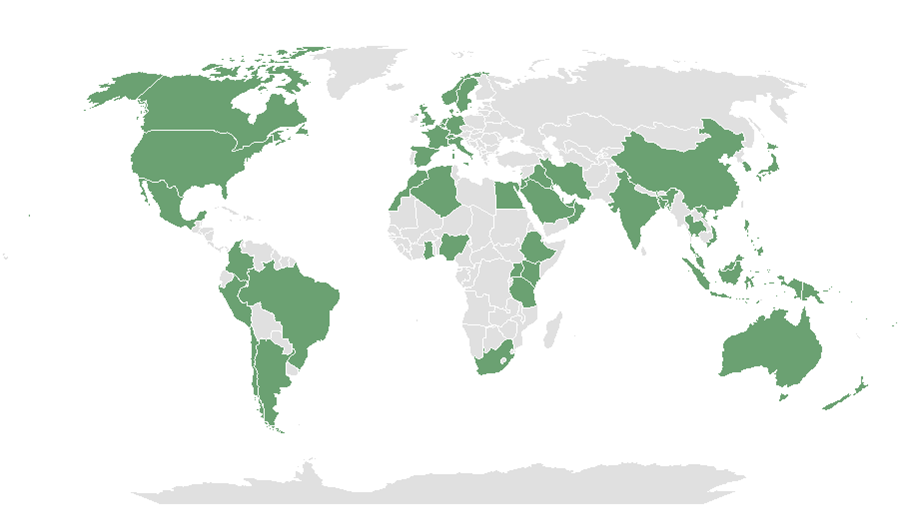
\includegraphics[width=0.8\linewidth]{figs/world_operations.png}
    \caption{Countries of operation of Forbes Marshall}
    \label{fig:world_operations}
\end{figure}

As of now, Forbes Marshall has established itself as a global leader in energy conservation and automation solutions. The company has a strong presence worldwide with 37 offices, 6 manufacturing units, and 18 distribution centers. This extensive network allows Forbes Marshall to effectively serve its diverse customer base.

To ensure excellent customer support, Forbes Marshall has a team of 500 dedicated sales and service engineers who work tirelessly to meet the needs of their 8,000 customers worldwide. The company values customer engagement and conducts 1,250 customer connects daily, fostering strong relationships and understanding their evolving requirements.

With a focus on continuous innovation, Forbes Marshall remains committed to research and development. The company's large R\&D team is dedicated to developing new products and services that address the industry's future needs. By prioritizing energy and process optimization, Forbes Marshall aims to reduce energy consumption and make a positive impact on the environment.

\subsection{Research and Development}
Forbes Marshall's deep customer knowledge and understanding of industry needs drive the development of new products and services. The company has a large Research \& Development team dedicated to innovating for the future needs of the industry. Through research-based innovations, Forbes Marshall continues to prioritize energy and process optimization, resulting in lower levels of energy consumption and a positive impact on the environment.

\subsection{Sustainability Initiatives}
\subsubsection{Energising Communities}
Forbes Marshall is committed to giving back to the communities where it operates. As part of its corporate social responsibility initiatives, the company partners with local organizations that focus on education for children, skilling for youth, and mobilizing women through self-help groups. These initiatives aim to empower individuals and contribute to the long-term wellness of families by providing healthcare services.

\subsubsection{Investing in a Better Future}
In 2012, Forbes Marshall established the Forbes Foundation to invest in organizations and strategic social innovation projects in Maharashtra, India, and beyond its immediate geographic communities. The foundation focuses on addressing issues in education, building resilience in communities, and supporting good governance. By investing in future innovations, Forbes Marshall aims to collaboratively tackle pressing societal issues that are often unsupported.

\subsubsection{Identifying Needs}
Forbes Marshall actively engages with community members to identify their needs and work towards achieving a common goal of creating an equitable society.

\subsubsection{Collaborating}
The company collaborates with organizations and community members to co-design, monitor, and support solutions that address the identified needs. By working together, Forbes Marshall aims to create sustainable and impactful change within the community.

\subsubsection{Catalyzing Change}
Forbes Marshall strives to build awareness, provide perspective, and offer access to resources that can catalyze positive change within the community. Through its initiatives, the company has touched the lives of 150,000 individuals, impacted 35,000 people through its corporate social responsibility efforts, supported 50 NGOs through cohorts and incubators, reached 4,000 students, and economically empowered 3,000 women.
